\subsection{Solución actividad 1}
2. El sistema representado en la Ecuación (39) es implementado en Simulink a través del código mostrado en la Fig. 37\\

\begin{center}
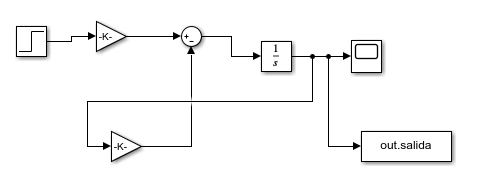
\includegraphics[scale=0.6]{actividad1Circuito.png} 
\end{center}

3. Coloque en el código en simulink una entrada tipo step con un valor inicial 0[u], un valor final 1[u] y un tiempo de desfasamiento de 0[s], observe y analice la respuesta obtenida en el osciloscopio.\\

\begin{center}
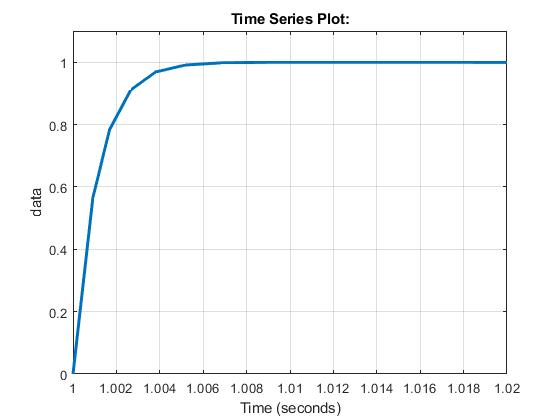
\includegraphics[scale=0.6]{actividad1R15000.jpg} 
\end{center}

\begin{verbatim}
R1=5000
C1=0.22e-06
\end{verbatim}

4. ¿Qué le pasa a la respuesta del sistema cuando se modifica el valor del parámetro $R_!$?

\begin{center}
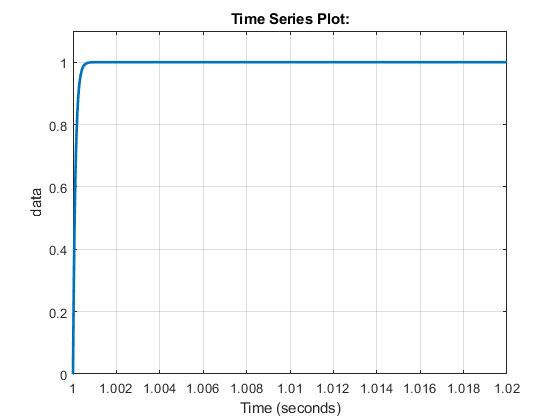
\includegraphics[scale=0.6]{actividad1R1500.jpg} 
\end{center}

\begin{verbatim}
R1=500
C1=0.22e-06
plot(out.salida,'linewidth',2)
axis([1 1.02 0 1.10])
grid on
\end{verbatim}

Podemos observar como llega más rápido al valor de saturación y = 1, es decir, cambia su tiempo de respuesta. Debido a la variación de la oscilación de la gráfica podemos ver que al disminuir la magnitud de la resistencia le estamos exigiendo demasiado al sistema.\\

5.Cambia el valor del parámtero $C_1$ y compara la respuesta obtenida con las anteriores. ¿Qué sucede?\\

\begin{center}
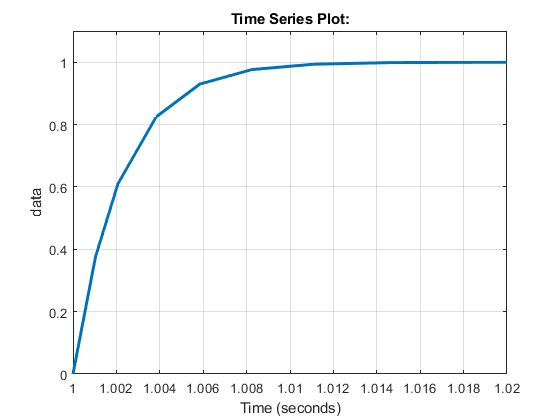
\includegraphics[scale=0.6]{actividad1C44.jpg} 
\end{center}

\begin{verbatim}
R1=5000
C1=0.44e-06
plot(out.salida,'linewidth',2)
axis([1 1.02 0 1.10])
grid on
\end{verbatim}

Nuevamente cambia el tiempo de respuesta del sistema. En este caso le toma más tiempo llegar al punto de saturación, y = 1, por lo que podemos decir que al aumentar la magnitud de la capacitancia estamos ayudando a que se le exija menos al sistema.\\
